\section{Soll-Zustand und Anforderungen}\label{sec:Soll}
%In diesem Kapitel wird der Soll-Zustand des Labormusters und des Demonstrators beschrieben. Dafür werden einzelne Themen aus dem Ist-Zustand herausgegriffen und für das Projekt Güterwagen 4.0 beschrieben.\par
In diesem Kapitel findet die Beschreibung des Soll-Zustandes gleichzeitig %Gleichzeitig findet die 
mit der Beschreibung der Anforderungen statt. Diese bestehen immer aus einer Anforderungsnummer und einem Anforderungstext sowie eventuell dazugehörigen Notizen.\par
%Die Anforderungen ergeben den Sollzustand.
Das Erkennen von Anforderungen ist auch Teil des Forschungsinhaltes des Projektes, so dass diese Auflistung keinen Anspruch auf Vollständigkeit hat.
\subsection{Allgemeines}
Für alle Aspekte ist eine spätere Zulassung des System zu berücksichtigen. Dem entsprechend ist auf eine Beachtung der folgenden Normen zu achten. Labormuster und \gls{Demonstrator} sind aber als Prototyp zu sehen, sodass bei einzelnen Prototypenentwicklungen auch davon abgewichen werden kann. \par
Alle Komponenten sind schwingungsarm unterzubringen. Dies soll, für den Demonstrator, die Möglichkeit geben auch Komponenten, die nicht aus dem Bahnbereich stammen, verwenden zu können.
\begin{feat}
Der \gls{Gueterwagen} muss alle Anforderungen an einen konventionellen Gü- terwagen ebenfalls erfüllen.
\end{feat}
\begin{feat}
Die \gls{40-Komponenten} auf dem \gls{Demonstrator} müssen vollständig abschaltbar sein.
\end{feat}
\begin{feat}
Die \gls{40-Komponenten} im \gls{Demonstrator} sind entweder selbst nach Schutzklasse IP 68 ausgerüstet oder danach zu schützen.
\end{feat}
\begin{feat}
Die \gls{40-Komponenten} auf dem \gls{Demonstrator} müssen vollständig nachrüst- bar sein.
\end{feat}
\begin{feat}
Für Zulassungen ist die CSM-VO - Verordnung (EG) Nr. 402/2013 anzuwenden.
\end{feat}
\begin{feat}
Die \acrshort{DIN} \acrshort{EN} 50155:2018 Bahnanwendungen - Elektronische Einrichtungen auf Schienenfahrzeugen ist - soweit anwendbar - anzuwenden.
\end{feat}
\begin{feat}
Die \acrshort{DIN} \acrshort{EN} 61373:2011-04 Bahnanwendungen - Betriebsmittel von Bahnfahrzeugen - Prüfungen für Schwingen und Schocken ist anzuwenden.
\end{feat}
\begin{feat}
Die Technische Richtlinie zur EMV Verträglichkeit TR-EMV ist anzuwenden.
\end{feat}
\begin{feat}
Die TSI ist für Brandschutz in Schienenfahrzeugen ist anzuwenden.
\end{feat}
\begin{rem}[zu Anf. 6-8]
Möglich wäre beispielsweise eine schwingungsarme Metallbox, die sowohl die EMV- als auch die Brandschutzrichtlinien erfüllt.
\end{rem}

\subsection{Energieversorgung}\label{sec:EV}
Die Energieversorgung des Bordnetzes erfolgt mittels Systembatterie. Diese wird durch externe Versorgung gespeist. Weil im Rahmen des F\&E-Projekts keine Umläufe mit kalkulierbarem Streckenanteil geplant sind, wird die Batterie in der Regel im Stand mit Hilfe eines Netzgerätes geladen. Der Demonstrator soll darüber hinaus die Möglichkeit der Aufladung durch einen Achsdeckelgenerator beinhalten (Anpassung für unterschiedliche Einspeisespannungen). Siehe dazu auch Abbildung \ref{fig:Soll-EV}. 
\begin{figure}[htp]
    \centering
    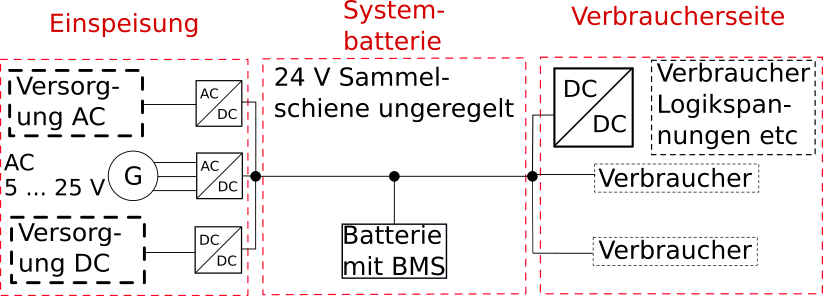
\includegraphics[width=\textwidth]{Bilder/20190706_SkizzeBatterieohneText.png}
    \caption{Beispielhafte Energieversorgung des Güterwagen 4.0}
    \label{fig:Soll-EV}
\end{figure}

\subsubsection{Spannungsversorgung}
\begin{feat}
Die Nennspannung des Systems ist mit 24 VDC vorzusehen
\end{feat}
\begin{rem}[zu Anf. 10]
Aufgrund der Prototypenentwicklung in diesem Projekt erscheint eine 24 V-Spannungsversorgung für dieses Projekt sinnvoll. Sowohl werden alle Grenzen der Berührspannungen im Kleinspannungsbereich eingehalten, als auch gibt es bereits sehr viele Produkte auf dieser Spannungsebene. Namentlich genannt die SPS, aber auch diverse Sensoren und Aktoren.
\end{rem}

\subsubsection{Einspeisung}
\begin{feat}
Es sind folgende externe Versorgungsmöglichkeiten für die \gls{Systembatterie} vorzusehen:
\begin{itemize}
    \item 100 - 240 VAC - Netzspannung mit Anpassungselektronik / Gleichsetzsteller
    \item Achsdeckelgenerator mit Anpassungselektronik
    \item Schnittstelle für DC-DC-Versorgung bspw. durch Solarpanels oder AK mit Anpassungselektronik
%    \item Weitere
\end{itemize}
\end{feat}

\subsubsection{Batterie}
%Gepuffert werden soll das System durch eine Batterie. Diese Batterie soll genügend Leistung liefern um sämtliche Daten-, Kommunikations- und Aktorsteuerungsprozesse speisen zu können. Außerdem soll sie genügend Energie für den Erprobungsbetrieb bieten.\par
%Die Batterie soll mittels Ladegerät von 230 V nachladbar sein, aber auch eine Schnittstelle für einen Achsdeckelgenerator bieten. Zum Aufladen wird dieser wahrscheinlich nicht geeignet sein, da keine entsprechenden Umlaufzyklen während der Testphase möglich sind. Die Batterie ist in einem Einschubkasten so anzubringen, dass sie von außen zugänglich, aber auch vor Steinschlag und ähnlichem während einer Fahrt geschützt ist.\par
\begin{feat}
Es ist eine \gls{Systembatterie} mit Batteriemanagementsystem vorzusehen.
\end{feat}
\begin{rem}[zu Anf. 10]1
Die Batterie soll genügend Leistung, Spannung und Energie für sämtliche Daten-, Kommunikations- und Aktorprozesse liefern.
\end{rem}
\begin{rem}[zu Anf. 11]
Die Batterie soll genügend Leistung, Spannung und Energie für den Erprobungsbetrieb haben.
\end{rem}
\begin{feat}
Für die Batterie ist ein Batteriekasten vorzusehen. 
\end{feat}
\begin{rem} [zu Anf. 12]
Das Fach ist so anzubringen, dass es von außen zugänglich, aber auch vor Schotterflug und ähnlichem während einer Fahrt geschützt ist und eine möglichst einfache Wartbarkeit ermöglicht.
\end{rem}
\begin{rem} [zu Anf. 12]
Zusätzlich muss die Befestigung des Kastens sicher und stoßgeschützt sein.
\end{rem}

\subsubsection{Anschlusskasten und Leitungen}
\begin{feat}
Es ist mindestens ein Anschluss- oder Klemmenkasten für die Spannungsversorgung von Sensoren und Aktoren vorzusehen. 
\end{feat}
\begin{feat}
An beiden Wagenenden ist ein Zugang zu den Daten- und Stromleitungen ist vorzusehen.
\end{feat}
\begin{feat}
Die Daten- und Stromleitungen sind geschützt in Stahlrohren zu verlegen.
\end{feat}

\subsection{Sensoren und Aktoren}
\begin{feat}
Sämtliche sicherheitskritische Informationen sind zweikanalig zu übertragen.
\end{feat}
\begin{feat}
Die Zustände aller Notbedienelemente sind zurückzumelden.
\end{feat}

\subsubsection{Pneumatische Bremse}
\paragraph{G/P-Umstellung}
\begin{feat}
Eine elektrisch gesteuerte Einstellung der Bremsstellung jedes Wagens ist vorzusehen.
\end{feat}
\begin{rem} [zu Anf. 19]
Dafür werden die Bremsstellungen G und P unterstützt.
\end{rem}

\paragraph{Lösen der Bremse}
\begin{feat}
Eine elektronische Betätigung des Lösezuges ist vorzusehen.
\end{feat}
\begin{rem}[zu Anf. 20]
Das bedeutet, die A-Kammer ist elektrisch gesteuert zu entlüften.
\end{rem}

\paragraph{Lastwechsel}
\begin{feat}
Falls erforderlich ist eine elektrische Einstellung des Beladungszustandes vorzusehen.
\end{feat}

\paragraph{Abschalten der Bremse}
\begin{feat}
Ein elektrisches Abschalten der kompletten Bremse ist vorgesehen.
\end{feat}

\paragraph{Aktoren in der Hauptluftleitung}
\begin{feat}
Die \acrshort{HL}-Endabsperrhähne sind durch elektrische Endabsperrhähne auszuführen. Diese sind bistabil und mit elektrisch betätigbarer Aktorik versehen. Zusätzlich verfügen sie über eine Notfbetätigungsmöglichkeit.
\end{feat}

\paragraph{C-Druck}
\begin{feat}
Der C-Druck ist in geeigneter Weise zu messen.
\end{feat}

\subsubsection{Feststellbremse}
\begin{feat}
Es ist eine elektronische Feststellbremse vorzusehen.
\end{feat}
\begin{rem}[zu Anf. 25]
Wechselwirkungen zwischen Feststellbremse und pneumatischer Bremse sind beim Anlegen und Lösen zu berücksichtigen.
\end{rem}

\paragraph{Außenanzeige}
\begin{feat}
Es sind geeignete Anzeigen für Endabsperrhähne, Bremsstellung, \gls{Lastwechsel} und der Feststellbremse zu sorgen vorzusehen. Diese sind als sichere Anzeigen auszuführen.
\end{feat}
\begin{feat}
Es ist für geeignete passive, mechanische Anzeigen zu sorgen.
\end{feat}

\subsubsection{Condition Monitoring}
\begin{feat}
Für das Condition Monitoring werden folgende Sensoren benötigt:
\begin{itemize}
    \item Lagertemperatur
    \item Beschleunigung in x-, y- und z-Richtung
    \begin{itemize}
        \item Zur Überwachung von: Stößen, Lagerzuständen und Flachstellen
    \end{itemize}
    \item Laufleistung / Radumdrehung / Drehzahl
    \item Gewicht der Ladung
    \item GPS
    \item Aktueller Radsatzdurchmesser
    \item Historie der Bremsvorgänge
\end{itemize}
\end{feat}

\subsubsection{Weitere Sensoren}
\begin{feat}
Weitere Benötigte Sensoren für den Forschungsbetrieb sind:
\begin{itemize}
    %\item Drucksensoren in der \acrshort{HL} an strategischen Stellen
    %\item Drucksensor R-Behälter
    \item Ladezustandsmessung der Batterie
    \item Lade- und Entladestrom
    \item Türschalter für aufgesetzten Container (Schnittstelle Ladung / Wagen)
\end{itemize}
Diese sind vorzusehen.
\end{feat}

\subsection{Fahrzeugsteuerung und -kommunikation}
Die Wagen kommunizieren untereinander. Eine gebildete Wagengruppe ist nach außen wie ein Wagen zu behandeln. Jeder Wagen in dieser Wagengruppe kann Informationen über jeden Wagen der Wagengruppe herausgeben.\par
Jede Funktion des Wagens wird durch ein Befehl der Steuerung veranlasst. Es gibt verschiedene Möglichkeiten der Initialisierung von Befehlen.\par
Grundsätzlich gibt es vier Kommunikationskanäle:
\begin{itemize}
    \item Kommunikation innerhalb des Wagens
    \item Kommunikation zwischen den Wagen
    \item Kommunikation im Nahbereich
    \item Kommunikation im Fernbereich
\end{itemize}

\subsubsection{Datenhaltung und -übertragung}
\begin{feat}
Alle Steuerbefehle müssen sicher und zuverlässig übertragen werden
\end{feat}
\begin{feat}
Sicherheitskritische und sicherheitsunkritische Funktionen und Anwendungen sind zu trennen.
\end{feat}
\begin{feat}
Die Reichweite soll für jeden Zweck ausreichend sein.%, aber von außen nicht stör- oder abhörbar.
\end{feat}
\begin{feat}
Die Daten sollen auf geeignete Weise verschlüsselt und vor Missbrauch nach aktuellem Stand der Technik geschützt sein.
Das IT-System ist für die entsprechenden Anwendungszwecke ausreichend sicher auszulegen.
\end{feat}
\begin{feat}
Die Bandbreite soll für jede Kommunikationsart ausreichend sein.
\end{feat}

\paragraph{Kommunikation innerhalb des Wagens}
\begin{feat}
Innerhalb des Wagenkastens werden alle Daten vorzugsweise kabelgebunden transportiert. 
\end{feat}

\paragraph{Kommunikation zwischen den Wagen}
\begin{feat}
Die Kommunikation zwischen den Wagen findet vorzugsweise in der Nähe der Puffer statt.
\end{feat}
\begin{feat}
Für eine Übertragung zum nächsten Wagen sind kurze Funkstrecken oder Kabel (nach UIC 568) vorzusehen.
\end{feat}
\begin{rem}[zu Anf. 37]
Kurze Funkstrecken können über
\begin{itemize}
    \item WLAN (60GHz),
    \item NFC,
    \item Bluetooth,
    \item ...
\end{itemize}
realisiert werden.
\end{rem}

\paragraph{Kommunikation im Nahbereich}
\begin{feat}
Eine Kommunikation zwischen Wagen / Wagengruppe und Bediener ist innerhalb vom drahtlosen Netzwerk möglich.
\end{feat}

\paragraph{Kommunikation im Fernbereich}
\begin{feat}
Eine Kommunikation mit der Cloud ist zum Beispiel über den Mobilfunk möglich
\end{feat}
\begin{feat}
Die Kommunikation muss rückwirkungsfrei sein. Es darf nur eine Leseberechtigung seitens der Cloud gewährt werden.
\end{feat}

\subsubsection{Autorisierung}
\begin{feat}
Es ist sicherzustellen, dass Bediener berechtigt sind.
\end{feat}
\begin{rem} [zu Anf. 41]
Es sind verschiedene Autorisierungsstufen vorzusehen. Jede Gruppe braucht eine ausreichende Zugriffsmöglichkeit auf benötigte Daten.\\
Autorisierungsstufen können zum Beispiel sein:
\begin{itemize}
    \item Stufe 1: Rangierpersonal in den Einfahrgruppen der Rangierbahnhöfe
    \item Stufe 2: Wagenmeister in Ausfahrgruppen
    \item Stufe 3: Notfallmanager auf freier Stecke
\end{itemize}
\end{rem}
\begin{rem} [zu Anf. 41]
Verschiedene Daten sollen nur in gewissen Geofencing-Bereichen abrufbar und veränderbar sein.
\end{rem}

\subsubsection{Bordrechner}
\begin{feat}
Es ist ein Bordrechner vorzusehen
\end{feat}
\begin{feat}
Der Bordrechner verfügt über genug Rechenleistung für die Verarbeitung sämtlicher auf dem Wagen vorhandener Daten sowie die Kommunikation mit weiteren Wagen, Anwendern und der ggf. Cloud.
\end{feat}
\begin{feat}
Der Bordrechner verfügt über genug Speicher für die Speicherung aller notwendigen Daten.
\end{feat}
\begin{feat}
Sichere und nicht sichere Funktionen und ihre Daten sind - sofern technisch möglich - physikalisch getrennt zu verarbeiten und zu speichern.
\end{feat}

\subsubsection{Pneumatische Bremse}
\paragraph{Bremsstellungen}
\begin{feat}
Folgende Regelungen gelten für die Bremsstellung:
\begin{itemize}
    \item Der Wagen soll nach Aufforderung seine Bremsstellung in den gewünschten Modus umstellen können.
    \item Der Wagen soll abgeschaltete Bremsen selbstständig melden.
\end{itemize}
\end{feat}
\begin{rem} [zu Anf. 46]
Die Bremsstellung ist sowohl für jeden einzelnen Wagen, als auch für Wagengruppen zugleich, einzustellen.
\end{rem}

\paragraph{Lösen der Bremse}
\begin{feat}
Das Lösen der Bremse darf nur außerhalb des \gls{Zugverband}es bei entlüfteter Hauptluftleitung möglich sein.
\end{feat}

\paragraph{Lastwechsel}
\begin{feat}
Folgende Regel gilt für die \gls{Lastwechsel}einstellung:
\begin{itemize}
    \item Der Wagen soll nach Aufforderung den \gls{Lastwechsel} selbst vornehmen können, oder
    \item über eine automatische \gls{Lastwechsel}einstellung verfügen
\end{itemize}
\end{feat}
\begin{feat}
Die Einstellung des Lastwechsels darf nur im Stand möglich sein.
\end{feat}

\paragraph{Aktorsteuerung in der Hauptluftleitung}
\begin{feat}
Die Position der Hähne ist sicherzustellen.
\end{feat}
\begin{feat}
Die Hähne müssen je nach Betriebsart in der richtigen Stellung stehen.
\end{feat}
\begin{feat}
Hier ist folgende Regelung für die Aktorsteuerung der Endabsperrhähne in der \acrshort{HL} vorzusehen:
\begin{itemize}
    \item Ist der Güterwagen luftgekuppelt, so ist das Ventil in der \acrshort{HL} im Normalzustand an der Seite offen.
    \item Ist der Güterwagen nicht luftgekuppelt, so ist das Ventil in der \acrshort{HL} im Normalzustand auf der Seite geschlossen.
\end{itemize}
\end{feat}
\begin{rem}[zu Anf. 52]
Wie die dazugehörigen Informationen bereit gestellt werden, ist noch unklar und soll erforscht werden.
\end{rem}
\begin{rem}[zu Anf. 52]
Weitere manuelle Steuerungen, beispielsweise für Ablaufberge oder manuelle Bremsproben sind vorzusehen.
\end{rem}

\subsubsection{Feststellbremse}
\begin{feat}
Die Feststellbremse ist vom Bordrechner zu steuern.
\end{feat}
\begin{feat}
Die Feststellbremse muss die Betriebszustände berücksichtigen und sicherfe Zustände gewährleisten.
\end{feat}
\begin{feat}
Folgende Regelung gilt für die Feststellbremse:
\begin{itemize}
    \item Die Feststellbremse ist gelöst, wenn der Wagen luftgekuppelt ist.
    \item Die Feststellbremse ist angezogen, wenn der Wagen nicht luftgekuppelt ist.
\end{itemize}
\end{feat}
\begin{rem} [zu Anf. 55]
Weitere manuelle Steuerungen sind mittels Endgerät oder \newline Schalter am Wagen schnell und sicher zu ermöglichen.
\end{rem}
\begin{feat}
Die Feststellbremse darf nur im Stillstand und wenn die HL leer ist, ansteuerbar sein.
\end{feat}


\subsubsection{Bremsprobe und Bremsberechnung}
\paragraph{Bremsprobe}
\begin{feat}
Folgende Regelungen gelten für die Bremsprobe:
\begin{itemize}
    \item Der Wagen soll selbstständig seine Bremsfähigkeit (in t und in \%) angeben
    \item Der Wagen soll selbstständig seine Bremsfähigkeit (in t und in \%) erproben
    %\item Der Wagen soll selbstständig eine Rückmeldung an ein passendes Gerät geben
    \item Der Wagen soll den Druckverlauf im Reservebehälter angeben können
    \item Der Wagen soll den Druckverlauf in der \acrshort{HL} angeben
    \item Der Wagen soll den C-Druckverlauf angeben
    \item Der Wagen soll den A-Druckverlauf angeben
\end{itemize}
\end{feat}
\begin{feat}
Eine vom Rechner gesteuerte automatische Bremsprobe ist möglich.
\end{feat}
\begin{rem} [zu Anf. 58] 
Der Rechner gibt die Bremshunderstel für die gegebene Konfiguration des \gls{Zugverband}es an.
%%%%%%%%%%%%%%%%%%%%%%
\begin{comment}
Diese hat sich für folgende Fahrten zu unterscheiden:
\begin{itemize}
    \item für Bedienfahrt
    \item für Rangierfahrt
    \item für Sperrfahrt
    \item für Zugfahrt
\end{itemize}
\end{comment}
%%%%%%%%%%%%%%%%%%%%
\end{rem}

\paragraph{Technische Wagenbehandlung}
\begin{feat}
So weit eine \gls{technische Wagenbehandlung} aktor- und sensorgeführt möglich ist, soll diese integriert werden.
\end{feat}
\begin{feat}
Es soll geprüft werden welche Schritte der Zugborbereitung durch die automatisierte \gls{technische Wagenbehandlung}  unterstützt werden können.
\end{feat}
%%%%%%%%%%%%%%%%%%%%%%%%
\begin{comment}

\begin{feat}
Folgende Regelungen gelten für die \gls{technische Wagenbehandlung}:
\begin{itemize}
    \item Hier muss was hin
\end{itemize}
\end{feat}
\end{comment}
%%%%%%%%%%%%%%%%%%%%%%%%%%

\paragraph{Bremsberechnung}
\begin{feat}
So weit eine Bremsberechnung aktor- und sensorgeführt möglich ist, soll diese integriert werden. Wie weit dies möglich ist, soll im Rahmen des Projektes geprüft werden
\end{feat}
%\begin{feat}Eine automatische Bremsberechnung anhand des Wagenzuges und der Lok ist möglich. \end{feat}
%\begin{rem} [zu Anf. 30]
%Die Regelungen zur Bremsberechung sind:
%\begin{itemize}
 %   \item ...
%\end{itemize}
%\end{rem}

%%%%%%%%%%%%%%%%%%%%%%%%%%%%
%Hier muss was hin.

\subsubsection{Wagentrennung und -zusammenstellung}
\begin{feat}
Eine elektrische Vorbereitung von Trennstellen ist möglich.
\end{feat}
\begin{rem} [zu Anf. 51]
Folgende Regelungen gelten für die Trennstellenanzeige:
\begin{itemize}
    \item Ist auf dem Endgerät eine Trennstelle angewählt, so müssen die \acrshort{HL}-Absperrventile sich an diesen Punkte schließen um eine Luftkupplungstrennung zu ermöglichen.
    \item Die Trennstellenanzeige muss deutlich von allen Seiten des Güterwagens sichtbar sein.
    \item Die Trennstellenanzeige muss farblich erkennbar sein.
\end{itemize}
\end{rem}
\begin{feat}
Eine automatische Wagengruppenbildung ist möglich.
\end{feat}
\begin{feat}
Die elektrische Vorbereitung von Kuppelstellen ist möglich.
\end{feat}
Die Vorprüfung der Wagen im automatisierten Rangierbahnhof sollen bei einem Wagenzug, der nur aus ausgerüsteten Güterwagen 4.0 besteht, nicht mehr notwendig sein, da dort die Reihenfolge der Wagen bekannt ist. Solange nicht alle Wagen Güterwagen 4.0 sind, muss dieser Prozess weiter ausgeführt werden.
\begin{feat}
Eine Überprüfung der Wagenreihung ist möglich.
\end{feat}
\begin{feat}
Eine Speicherung des technischen Zustands aus vorheriger Fahrt ist \newline wünschenswert.
\end{feat}
\begin{feat}
Eine automatische Übermittlung von Transportunterlagen ist\newline möglich.
\end{feat}
\begin{feat}
Auf dem Wagen soll ein elektronischer Frachtbrief digital vorhanden und abrufbar sein.
\end{feat}

\subsection{Diagnosefunktion}
Die Diagnosefunktionen sind Teil der Forschung. Der Wagen soll mit Hilfe von wissensbasierten Diagnosen die Zugvorbereitung unterstützen. In wie weit das möglich ist, soll im Projekt untersucht werden. 
\begin{feat}
Alle für eine vorausschauende Wartung notwendigen Sensoren sollen eingebaut und überwacht werden.
\end{feat}
\begin{feat}
Für eine Prognose der Sicherheit der Lastzyklen sind Lade- und Entladestrom zu messen und auszuwerten
\end{feat}
\begin{rem}
Sollten die gesammelten Daten der \gls{Demonstrator}en nicht ausreichend sein, so sind Daten zu simulieren.
\end{rem}
\begin{feat}
Diese Informationen soll der Wagen über sich speichern und abrufbar bereithalten.
\end{feat}
\begin{feat}
Alle bereits über den Wagen vorhandenen Informationen, wie Wartungszyklen, Instandhaltungen und ähnliches sollen als Dokument lokal auf dem Wagen  verfügbar sein.
\end{feat}

\subsection{Sonstiges}
\paragraph{Migrationsstrategie}
\begin{feat}
Eine Migrationsstrategie ist zu planen.
\end{feat}
\paragraph{Beladung und Ladungssicherung}
Hier sind für den \gls{Demonstrator} keine Änderungen geplant.
\paragraph{Mechanische und Luftkupplung}
Beim \gls{Demonstrator} ist keine Automatisierung der mechanischen oder der Luftkupplung geplant.
